%----------------------------------------------------------------------------
\chapter{Mérések}
\label{sec:results}
%----------------------------------------------------------------------------

A következő fejezetben szeretném bemutatni, hol és hogyan készültek a mérési eredmények, azokból mi olvasható ki. Fontos megjegyezni, hogy komolyabb mérések még a diplomamunka hátralevő részére vannak ütemezve, az alább bemutatott eredmények a rendszer működőképességét igazolják és némi előretekintést nyújtanak.

%----------------------------------------------------------------------------
\section{Mérés környezete}
%----------------------------------------------------------------------------
A feladat elején főként implementációval kellett foglalkozni így nem kapott jelentős szerepet a Kubernetes klaszter. Ezért  a félév első felében elég volt lokálisan futtatni, amit én Minikube (v1.17.1) segítségével tettem meg. 

Amikor a fejlesztési rész kezdett véglegesedni kellett egy rendes környezet, a rendes mérésekhez. Ehhez több lehetőséget is számításba vettem.	

\begin{itemize}
  \item \textbf{BME Cloud}: Egyik lehetőség az egyetemi felhő volt. Itt létre lehet hozni virtuális gépeket, amiket aztán klaszterbe lehet szervezni. Hátránya viszont, hogy hosszabb távra nehezen lehet gépet igényelni, rendszeresen le is állítják ami könnyen okozhatja egy-egy mérés elvesztését, hiszen több órán keresztül is futhat.
  \item \textbf{Klaszter a felhőben}: Kézenfekvő megoldás lehet igényelni egy teljes, egész klasztert. Erre több opció is van, csak hogy a legnagyobbakat említsem: Google, Amazon, Microsoft. Ezek a minőségi szolgáltatások azonban havidíjasok lennének, és bizonyos tekintetben kevésbé rugalmasak. TODO: készültek becslések a havidíjra.
    \item \textbf{Tanszéki infrastruktúra}: A tanszéken létezik egy előretelepített klaszter, amin lehetne méréseket készíteni, de általában foglalt.
      \item \textbf{VM igénylés a Schönherz kollégiumtól}: A Villamosmérnöki és Informatikai Karhoz tartozó Schönherz kollégiumban lévő Kollégiumi Számítástechnikai Körtől lehet tanulmányokhoz és egyéb projekthez kapcsolódóan virtuális gépeket igényelni. Az igénylés leadása után lehetőséget kaptam három virtuális gép használatára egészen a projektfeladat végéig. Bizonyos hátulütőkkel ezen lehetőségnél is számításba kellett venni. Ilyen például, hogy öntevékeny körként hiba esetén a többinél lassabb válaszidőkre lehet számítani.
\end{itemize}		

A fenti opciók közül számomra a negyedik volt a legszimpatikusabb így kaptam is három teljesen új virtuális gépet. Telepítéshez a Debian (v10 - Buster) operációs rendszert választottam, mert stabil, megbízható és széles körben támogatott. A virtuális gépek tulajdonságai az \ref{tab:nodes} ábrán láthatóak. Hasonló erőforrásértékekkel rendelkeznek, annyi különbséggel, hogy csak az egyik gépnek van publikus címe. Továbbá a táblázat tartalmazza az egyes csomópontok nevét és a klaszteren belüli szerepét is.

\begin{table}[ht]
\centering
  \begin{tabular}{c|cccc}
	  Tulajdonság & VM 1 & VM 2 & VM 3 \\
    \hline
	CPU (mag) & 4 & 4 & 4 \\ 
	Memória (GB) & 4 & 4 & 4 \\
	Tárhely (GB) & 10 & 10 & 10 \\  
	Node neve & dipterv1 & dipterv2 & dipterv3 \\ 
	Külső IP & 152.66.211.2 & $\varnothing$ & $\varnothing$ \\ 
	Belső IP & 10.151.103.1 & 10.151.103.2 & 10.151.103.3 \\
	K8s szerep& control-plane,master & worker & worker \\
  \end{tabular}
  
  \caption{Használt csomópontok tulajdonságai}
\label{tab:nodes}
\end{table}

\subsection{Klaszter előkészítése}
%----------------------------------------------------------------------------
A virtuális gépekből klasztert kellett szervezni, amire különböző megoldások léteznek.\citep{kubernetesInstall} Két különbözőt szeretnék kiemelni:
\begin{enumerate}
  \item \textbf{Kubespray}: \textit{Ansible} felhasználásával előre definiált lépéseket hajt végre. Mindössze egy pár soros konfigurációt kell írni hozzá és ígérete szerint minden mást elintéz.
  \item \textbf{Kubeadm}: Az előzőhöz képest a \textit{kubeadm} jóval manuálisabb módszer. Segítségével le tudunk generálni mindenféle kulcsot a klaszterhez, csomópontokat bekötni a rendszerbe.
\end{enumerate}

Nem szándékosan de kipróbáltam mindkét megoldást. Vonzó volt ugyanis a Kubespray, hogy könnyen és automatikusan telepít minden függőséget. Sajnos pont amiatt mert ilyen magas szinten vezeti a telepítést hiba esetén nem sok információ derült ki. Miután eredménytelenül zárult minden próbálkozás, újratelepítettem a virtuális gépeket és áttértem a Kubeadm használatára. 

A telepítés menetét nem részletezném, mert a hivatalos weboldalon látható lépéseken kellett végigmenni. Az elkészült klaszter egy mester csomópontot és kettő kiszolgáló csomóponttal rendelkezik. A fő csomópont rendelkezik egyedül külső hálózatról elérhető, publikus IP címmel, a többinek csak belső címen érhetőek el. Ez némiképpen nehezítette a telepítés folyamatát, részben emiatt sem működött a Kubespray megoldása. 

A klaszter elkészülte után még pár függőséget ki kellett elégíteni, hogy a lokálisan összeállított mérő keretrendszer működni tudjon. Külön telepíteni kellett egy konténer hálózati interfészt (CNI). Ez alapból nem jön a Kubernetessel így külön kell installálni, hogy a különböző csomóponton futtatott konténerek tudjanak egymással kommunikálni. A választás a \textit{Cilium} szoftverre esett, mert szerettem volna jobban megismerni, széleskörűen használható és jól dokumentált. Telepítése után lehetőségünk van teszteseteket futtatni, ami igazolja a klaszterben a csomópontok és kapszulák kommunikációját. 

A \ref{sec:measure_orchestrate} szakaszban leírt módon a mérések során gyűjtött adatok jelentős részét a Prometheus rendszere gyűjti össze és tőle kérdezzük le. Emiatt az éles méréseket végző klaszterben is telepíteni kellett. Ebben a Helm, Kuberneteshez készített csomagkezelő megoldása segített. A \verb+prometheus-stack+ csomagot kellett telepíteni annyi kiegészítéssel, hogy kintről is elérhetővé tegyük a felületet és szolgáltatásait. Azt úgy érhetjük el, hogy a létrehozandó \verb+Service+  típusát \verb+NodePort+-ra állítjuk és a következetesség miatt adunk neki egy portszámot. Az így létrehozott környezet rendelkezik egy webes felhasználói felülettel is, ahol tetszőleges lekérdezéseket indíthatunk. Egy ilyen lekérdezés látszik az \ref{fig:prometheus_example} ábrán is. A példán az látszik, hogy milyen eredményt kapunk, ha lekérdezzük az aktuálisan futó kapszulákat a \verb+Default+ és \verb+Metrics+ névtérben. Az eredményből leolvasható, hogy jelenleg 3 darab \textit{back-end}, 2 darab \textit{front-end} és 1 darab \textit{db} névvel ellátott konténer fut. \\

% Prometheus példa -------------------------------------------------------
\begin{figure}[!ht]
\centering
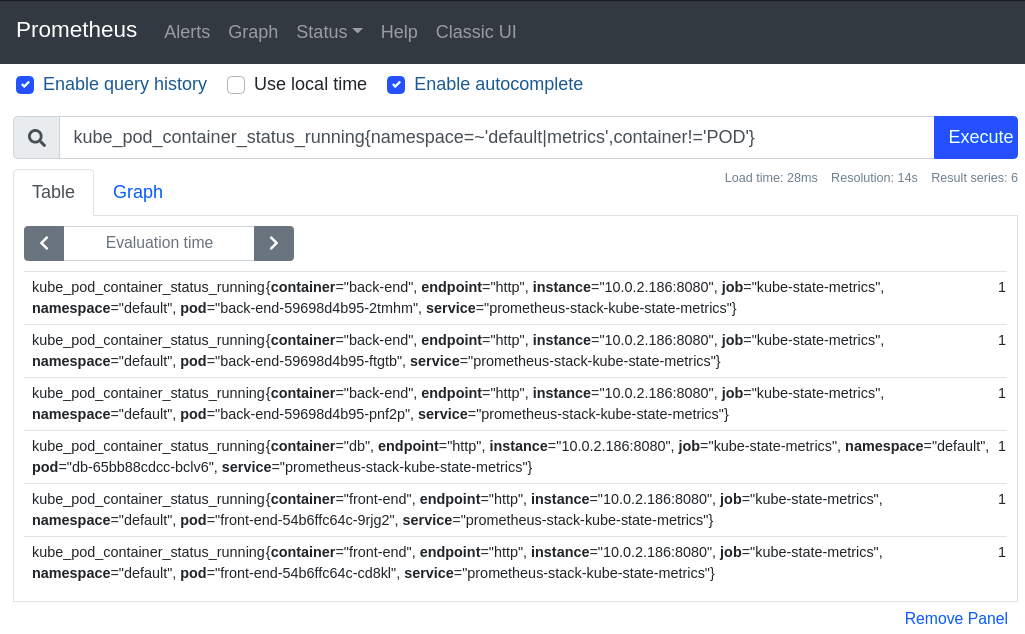
\includegraphics[width=150mm, keepaspectratio]{figures/prometheus_example.png}
\caption{Telepített \textit{Prometheus} rendszere}
\label{fig:prometheus_example}
\end{figure}

Az aktuális rendszerben az operátor még nem külön konténerként fut egy kapszulában, hanem a klaszteren kívül, lokálisan a szerveren, mint egy Go alkalmazás. Emiatt külön telepíteni kellett a Go nyelvet is, hogy el tudjon indulni a rendszer.

\subsection{Verziók}
%----------------------------------------------------------------------------
A rendszer és mérések összeállításához sok különböző komponenset kellett integrálni. Az \ref{tab:versions} táblázat összefoglalóan tartalmazza az egyes környezetek és használt eszközök verzióit. 

\begin{table}[ht]
\centering
  \begin{tabular}{l l}
	  Szoftver 		& Verzió \\
    \hline
      Go 			& 1.16.3 \\ 
      Kubernetes 	& 1.21.0 \\ 
      Kubectl 		& 1.21.0 \\
      Cilium 		& 1.9.5 \\
      Python 		& 3.7.3 \\ 
      Prometheus 	& 2.24.0 \\ 
      Grafana 		& 7.5.3 \\ 
      Operator-SDK 	& 1.4.0-32 \\ 
      Debian 		& 10 (buster)  \\ 
      Istio			& 1.11.4 \\
  \end{tabular}
  
  \caption{Használt verziók}
\label{tab:versions}
\end{table}


%----------------------------------------------------------------------------
\section{Eredmények kiértékelése}
%----------------------------------------------------------------------------
Az egyes méréseknek a kimenete egy-egy \textit{json} fájl, azonban ebből nem nagyon tudunk használható következtetéseket kiolvasni. Szükségessé vált egy külön alkalmazás implementálása, ami az általunk elkészített mérések eredményét fel tudja dolgozni. 

A feladat megoldására szintén a Python nyelvet választottam, mert könnyen lehet benne a \textit{json} objektumokat beolvasni és feldolgozni.
Fontos szempont volt, hogy minél könnyebben használható legyen az alkalmazás, így bizonyos paramétereket akár parancssorban is meg lehet adni. Ez látható az \ref{python_drawer} kódrészleten. Indításnál megadhatjuk, hogy milyen nevet szeretnénk a grafikonnak, milyen címke legyen az $X$ és $Y$ tengelyeken, hogy le akarjuk-e menteni az ábrát, illetve a legfontosabb, hogy melyik mappában keresse a mérési eredményeket. Egy példa konfiguráció is látható a korábban hivatkozott kódrészlet alján. \\

% Rajzoló program indítása --------------------------------------------------
\lstset{caption=Eredményeket feldolgozó alkalmazás használata, label=python_drawer}
\lstinputlisting{figures/python-drawer.sh}

Az alkalmazás indításakor meg kell adni, hogy hova vannak mentve a korábbi mérések során készült kimeneti fájlok. Itt egy-egy mérés jelentése, hogy a Fortio adott darabszámú lekérdezést generál másodpercenként fix ideig. Tehát egy teszteset futtatása több ilyen értelemben vett mérést tartalmaz, hiszen egy skálán megy végig a rendszer, ahol a minimális QPS értéktől megadott lépésközzel halad a maximális QPS értékig. 
Egyesével elkezdi beolvasni a mérési eredményeket és minden fájlból készít egy "tisztázott" eredményt. Ebben már csak az adott grafikon kirajzolásához nélkülözhetetlen értékeket tartalmazza. Például előfordul, hogy a Prometheus eredményében szerepel olyan pod is, ami nem vett részt az adott mérésben, mert még a korábbiból maradt ott. Az ilyen eseteket észlelni kell és kiszedni az értékeit, ne okozzanak anomáliákat. 

%----------------------------------------------------------------------------
\section{Példa mérés}
%----------------------------------------------------------------------------
A rendszer összeállítása után méréseket is lehet már végezni. A mérés mérésben két szolgáltatás vett rész, ahogy az az \ref{fig:sample_sg} sorszámú ábrán is látszik. A szolgáltatáshálóban két különböző feladatot ellátó szolgáltatás szerepelt. Volt egy nodeport segítségével kintről elérhető \textit{front-end} szolgáltatás, illetve egy csak bentről elérhető \textit{back-end}. Azt a szituációt vizsgáltuk, amikor a \textit{front-end} nem használ sok erőforrást, és két pod fut belőle. Ezzel szemben a \textit{back-end} egy jóval erőforrásabb szolgáltatás, cserébe három egység fut belőle. A \textit{front-end} minden felé érkező, \verb+/to-backend+ végpontra érkező kérést továbbított a \textit{back-end} \verb+heavy+ végpontjára. Ezzel elértük, hogy a második szolgáltatásunk a számára beállított, sok processzort igénylő műveletet hajtsa végre.


% Példa szolgáltatás háló----------------------------------------------------
\begin{figure}[!ht]
\centering
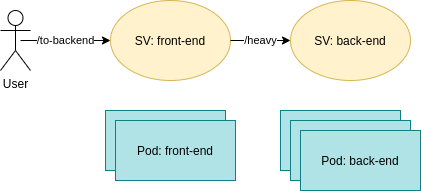
\includegraphics[width=100mm, keepaspectratio]{figures/sample_measurement.png}
\caption{A mérésnek kitett szolgáltatások kapcsolata}
\label{fig:sample_sg}
\end{figure}

A kapott eredményekből készült grafikon látható az \ref{fig:example_plot} és \ref{fig:example_responsetime} ábrán. 

A kapott \ref{fig:example_responsetime} ábráról leolvasható, hogy az átlagos válaszidő a mérés során nem változott érdemben, végig kellően alacsony maradt. Fontos megjegyezni, hogy a mérés során nem vittünk a rendszerbe mesterséges késleltetést, csak a kötelező műveletek elvégzését vártuk meg, így jött ki az állandó válaszidő.

A másik, \ref{fig:example_plot} grafikonon látható, hogy a kevésbé erőforrás-igényes \textit{front-end} processzor felhasználása lassan de folyamatosan nő egészen addig, amíg a \textit{back-end} is tudja növelni a processzor felhasználását. Ez körülbelül 125 QPS-ig tart. Ilyenkor a \textit{back-end} eléri az indításkor beállított erőforrás limitációt és emiatt nem tud több beérkező igényt kiszolgálni.  Emiatt a felhasználói forgalmat generáló Fortio sem fog tudni több kérést a rendszer felé küldeni, mert meg kell várja, mire a \textit{front-end} válaszol, de a front-end csak azután válaszol, hogy meghívta a végletekig megterhelt \textit{back-end} szolgáltatást.

Érdemes figyelembe venni, hogy az $X$ tengely az igényelt lekérdezések darabszámát mutatja, nem a rendszer által valóságban kiszolgált kérések mennyiségét. \\


% Generált példa ábrák -------------------------------------------------------
\begin{figure}[!ht]
\centering
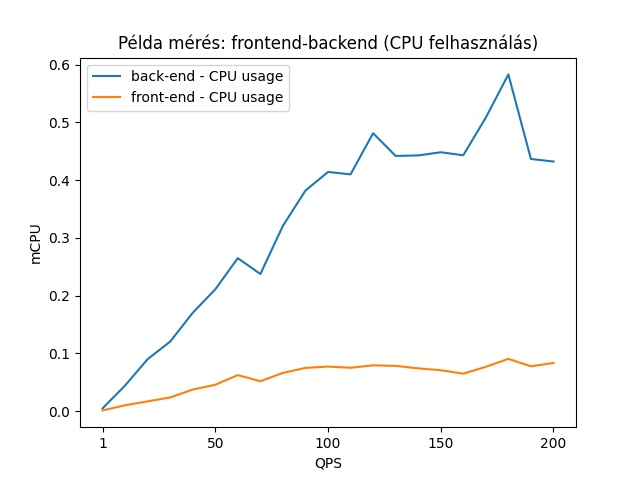
\includegraphics[width=150mm, keepaspectratio]{figures/sample_plot_cpu.jpg}
\caption{\textit{Front-end} és \textit{back-end} egységből álló rendszer CPU felhasználása}
\label{fig:example_plot}
\end{figure}

\begin{figure}[!ht]
\centering
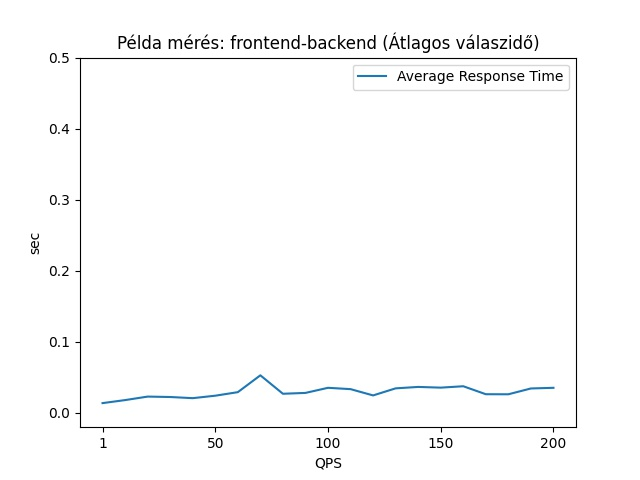
\includegraphics[width=150mm, keepaspectratio]{figures/sample_plot_responsetime.jpg}
\caption{\textit{Front-end} és \textit{back-end} egységből álló rendszer átlagos válaszideje}
\label{fig:example_responsetime}
\end{figure}


%----------------------------------------------------------------------------
\section{Finomhangolás}
%----------------------------------------------------------------------------
Az eredmények megjelenítésén még lehetne finomítani, mivel jelenleg egy grafikonon csak egy mérési sorozat kimenetét dolgozzuk fel. Ez viszont azzal jár, hogy az egyes mérések során lehetségesek eltérések. Például ilyen lehet, hogy a Prometheus még nem tudta lekérdezni az összes konténer utolsó erőforrás-használatait. A probléma orvoslására jelenleg biztonsági időket iktattunk be a mérés során, hogy minimalizáljuk ennek az esélyét. A szebb megoldás viszont az lenne, ha több mérést végeznénk azonos feltételek mellett és ezeknek az átlagát vennénk figyelembe.

Illetve érdemes elgondolkodni, hogyan kellene kezelni az esetet, ha a rendszer nem tudja kiszolgálni az elvárt lekérdezéseket. Több megoldás is szóba jöhet. Egyik, hogy már a mérések végzése folyamán figyeljük és ha nem tudja teljesíteni, akkor idő előtt leállítjuk a terheléseket. Másik, hogy az $X$ tengelyen a valódi, kiszolgált QPS értéket jelenítjük meg. Ezzel annyi gond lehet, hogy elveszítjük az információt, hogy az adott mérésnél a rendszer már túlterhelt állapotban volt és emiatt vagy alapból ennyi kéréssel terheltünk. Harmadik megoldás, hogy az $X$ tengelyen lévő értékeket addig ábrázoljuk, amíg elvárt módon futottak a mérések.

Másik apróság, ami segítene az eredmények vizualizációjában, ha a felhasznált erőforrások és a hozzá kapcsolódó válaszidő egy ábrán lenne, viszont ehhez külön $Y$ tengely fog kelleni, hiszen más a mértékegysége.  

%----------------------------------------------------------------------------
\section{Tervezett mérések}
%----------------------------------------------------------------------------
A korábban bemutatott eredmények alapján a rendszerrel képesek vagyunk méréseket végezni az elvárt módon. Egyenlőre a kapott eredményekből még nem lehet nagyobb következtetéseket levonni, azonban segítség volt megtervezni a következő mérések környezetét. 

Jelenleg a Fortio az alapbeállításokkal indul el, ami 4 felhasználót szimulál. Emiatt tapasztaltuk az, hogy miután a \textit{back-end} telítésbe ment nem érkezett a \textit{front-end} felé több lekérdezés ami tovább tudta volna használni az erőforrásokat.  Szerencsére a könnyen módosíthatjuk ezt a beállítást és tetszőleges számú felhasználót (thread) tudunk majd szimulálni. Érdemes lehet majd ezt is külön paraméterként kivezetni a mérés konfigurációjába.

\begin{itemize}
\item \textbf{1 front-end, 1 back-end, 1 thread} - Ez lenne a legegyszerűbb eset. Később össze lehet hasonlítani a komplexebb mérési környezetekkel.
\item \textbf{1 front-end, 1 back-end, ~100 thread} - Várhatóan érdekesebb eredményeket fog hozni, mert ebben az esetben hiába lesz telítésben a \textit{back-end} a \textit{front-end} még fogadni fogja a többi felhasználó kéréseit, ami így várhatóan a \textit{back-end} előtt fel fog torlódni.
\item \textbf{Előző mérések, csak proszesszorigényes front-end} - Az előző méréseket meg lehet ismételni, csak más szolgáltatáshálón. Ebben az esetben a \textit{front-end} lenne az erőforrásigényes és a \textit{back-end} a könnyen kiszolgálható. Ebben az esetben már a \textit{front-end} előtt el kell dobódni a lekérdezéseknek.
\item \textbf{Horizontális skálázóval} - Miután megvannak a fenti mérések el tudjuk dönteni, hogy milyen eseteket érdemes megismételni és kiegészítve a horizontális pod skálázóval.
\end{itemize}

%----------------------------------------------------------------------------
\section{Elvégzett mérések}
%----------------------------------------------------------------------------
A projektmunka jelentős részét tette ki, hogy méréseket kellett végezni a korábban bemutatott rendszerelelmekkel rendelkező környezetben.
A mérések darabszámát szemlélteti \aref{python_drawer} kódrészlet. Beépített Linux parancsok segítségével könnyen megkaphatjuk a projekt során készített és a kiértékeléshez használt \textit{json} dokumentumok darabszáma. Ahogy a kódrészlet is mutatja először rekurzívan lekérdezzük az adott mappán és almappákon belül található adott kiterjesztéssel rendelkező fájlokat \textit{(find)}. 
Majd az így kapott eredményt csővezeték segítségével hozzákötjük egy szintén beépített parancs \textit{(wc)} bemenetére, ami megszámolja a kiírt sorok számát. 
Ahogy az a kódrészleten is látszik, hogy ennek a kimenete TODO $1445$, ami azt jelenti, hogy a projekt jelenlegi állapotához kapcsolódóan ennyi mérés született. 
Az egyes mérések itt egy-egy Vegeta terheléshez kapcsolódó konfigurációk, válaszidők és egyéb Prometheus-ból kapott eredményeket jelenti.

% Rajzoló program indítása --------------------------------------------------
\lstset{caption=Elvégzett mérések száma, label=number_of_measurements}
\lstinputlisting{figures/get_number_of_measuremnts.sh}